\section{Teorijske osnove i srodni radovi}
\label{chap:teorija}

Ovo poglavlje pruža sveobuhvatan pregled temeljnih teorijskih koncepata koji čine okosnicu predloženog modela optimizacije. Započet će se s formalizacijom problema odabira projektnog portfelja kroz analogiju s klasičnim problemom ruksaka. Zatim slijedi detaljna razrada genetskih algoritama kao odabrane optimizacijske metaheuristike, s posebnim osvrtom na njihove ključne komponente i više-kriterijsku inačicu NSGA-II. Poglavlje se nastavlja analizom Monte Carlo simulacije kao alata za kvantifikaciju rizika, te završava opisom metoda za modeliranje nesigurnosti projektnih aktivnosti.
\subsection{Problem odabira portfelja kao Knapsack problem}

Problem ruksaka (engl. \textit{Knapsack Problem}) jedan je od najpoznatijih problema kombinatorne optimizacije, svrstan u klasu NP-teških problema. Ta klasifikacija implicira da ne postoji poznati algoritam koji bi ga mogao riješiti u polinomnom vremenu, što znači da se vrijeme potrebno za pronalaženje optimalnog rješenja drastično povećava s veličinom problema \cite{GareyJohnson1979, Kellerer2004}. U svojoj osnovnoj, jednodimenzionalnoj verziji (0/1 Knapsack Problem), cilj je odabrati podskup objekata iz danog skupa, od kojih svaki ima definiranu težinu i vrijednost. Optimizacijski zadatak je maksimizirati ukupnu vrijednost odabranih objekata, pod uvjetom da njihova ukupna težina ne prelazi unaprijed zadani kapacitet "ruksaka". Formalno, za skup od n objekata, gdje svaki objekt i ima težinu $w_i$ i vrijednost $v_i$, te uz zadani kapacitet ruksaka W, cilj je maksimizirati funkciju:
$$
\max \sum_{i=1}^n v_i x_i \quad \text{uz ograničenje} \quad \sum_{i=1}^n w_i x_i \leq W, x_i \in \{0,1\}
$$
gdje je $x_i=1$ ako je objekt i odabran, a $x_i=0$ ako nije.

Ova elegantna formulacija čini ga moćnim alatom za modeliranje problema alokacije resursa. U kontekstu upravljanja projektima, problem odabira portfelja prirodno poprima oblik višedimenzionalne varijante (\textit{Multi-Dimensional Knapsack Problem} - MDKP). Ovdje projektne aktivnosti predstavljaju "objekte", a njihova vrijednost je povrat na investiciju (ROI). "Težina" aktivnosti nije jedna dimenzija, već vektor koji opisuje potrošnju različitih resursa – budžeta, radnih sati, itd. MDKP stoga pruža robustan matematički okvir za rješavanje središnjeg problema ovog rada. Postoji i niz drugih varijanti, poput problema neograničenog ruksaka (gdje se svaki objekt može uzeti više puta) ili višekriterijskog problema ruksaka (gdje se optimizira više ciljeva, npr. vrijednost i volumen), što dodatno pokazuje fleksibilnost ovog modela.

\subsection{Genetski algoritmi kao metaheuristika za pretraživanje}
\label{sec:ga}
Genetski algoritmi (GA) su moćne metaheurističke metode optimizacije temeljene na principima prirodne evolucije i genetike, koje je prvi formalizirao John Holland \cite{Holland1975}. Pripadaju široj klasi evolucijskih algoritama i iznimno su učinkoviti u rješavanju složenih optimizacijskih problema, posebno onih NP-teških, gdje klasične metode nisu praktične \cite{Gandomi2013, Mitchell1998}. Hollandova temeljna ideja bila je stvoriti računalni sustav koji oponaša najmoćniji proces rješavanja problema poznat u prirodi: evoluciju. Cilj je bio postići robustnu pretragu balansirajući dva ključna elementa: \textbf{iskorištavanje (exploitation)} postojećih dobrih rješenja i \textbf{istraživanje (exploration)} novih, potencijalno boljih dijelova prostora rješenja.
\subsubsection{Osnovni principi i tijek algoritma}

Umjesto pretraživanja prostora rješenja s jednom točkom, genetski algoritmi operiraju nad cijelom populacijom potencijalnih rješenja (kromosoma). Taj proces započinje generiranjem početnog, najčešće nasumičnog skupa rješenja, čime se osigurava početna raznolikost. Zatim ulazi u iterativnu petlju evolucije kroz generacije. U svakoj generaciji, svakom se rješenju (jedinki) dodjeljuje vrijednost pogodnosti (\textit{fitness}) koja kvantificira njegovu kvalitetu. Nakon evaluacije, provodi se selekcija, gdje jedinke s boljim fitnessom imaju veću vjerojatnost da budu odabrane kao "roditelji".

Ključna hipoteza na kojoj se temelji uspjeh GA, kako ju je popularizirao Goldberg \cite{Goldberg1989}, jest \textbf{hipoteza o građevnim blokovima (\textit{Building Block Hypothesis})}. Ona pretpostavlja da se dobra rješenja sastoje od manjih, visoko prilagođenih segmenata (građevnih blokova). Uloga genetskih operatora je upravo da kroz rekombinaciju i mutaciju otkrivaju i spajaju te blokove u sve kvalitetnije cjeline. Roditelji se rekombiniraju pomoću operatora križanja (\textit{crossover}), stvarajući "potomke" koji nasljeđuju i kombiniraju njihove karakteristike. Kako bi se održala raznolikost i izbjeglo zaglavljivanje u lokalnim optimumima, na potomke se primjenjuje operator mutacije. Na kraju, nova generacija potomaka zamjenjuje staru, i cijeli se proces ponavlja dok se ne zadovolji kriterij zaustavljanja \cite{Goldberg1989, Mitchell1998}.
\subsubsection{Ključni operatori i komponente}

Uspješnost genetskog algoritma ovisi o pažljivom odabiru i implementaciji njegovih ključnih komponenata ,čiji su temelji detaljno opisani u literaturi\cite{Goldberg1989}:

\paragraph{Reprezentacija rješenja i funkcija pogodnosti.} Prvi korak je definiranje načina na koji se rješenje problema kodira u kromosom. Za problem odabira portfelja, prirodan izbor je binarni niz, gdje svaki bit odgovara jednoj aktivnosti. Funkcija pogodnosti je ključna komponenta jer predstavlja vezu između problema i algoritma; ona uzima kromosom kao ulaz i vraća numeričku vrijednost njegove kvalitete.

\paragraph{Selekcija.} Operator selekcije oponaša prirodni odabir, dajući prednost jedinkama s višim fitnessom. Postoje brojne metode, poput popularne \textbf{selekcije metodom ruleta}, gdje svaka jedinka dobiva "dio" ruleta proporcionalan svom fitnessu. Iako je intuitivna, ova metoda može patiti od prerane konvergencije ako jedna jedinka ima dominantno visok fitness. Zbog toga se u praksi često koristi **turnirska selekcija**, odabrana i za ovaj rad. U njoj se nasumično odabire manja grupa jedinki ("turnir"), a pobjednik (jedinka s najboljim fitnessom) postaje roditelj. Veličina turnira, kako ističe Goldberg \cite{Goldberg1989}, jednostavno definira "selekcijski pritisak" – veći turnir znači veći pritisak i bržu konvergenciju, ali i veći rizik od gubitka raznolikosti.

\paragraph{Križanje (Crossover).} Križanje je glavni mehanizam iskorištavanja i rekombinacije, direktno povezan s hipotezom o građevnim blokovima. Dva roditeljska kromosoma razmjenjuju dijelove genetskog materijala kako bi stvorili potomke. Križanje u dvije točke, korišteno u ovom radu, odabire dva loma i razmjenjuje središnji segment, što se, prema Goldbergu, često pokazalo boljim za očuvanje dobrih kombinacija gena smještenih u sredini kromosoma.
\begin{figure}[H]
    \centering
    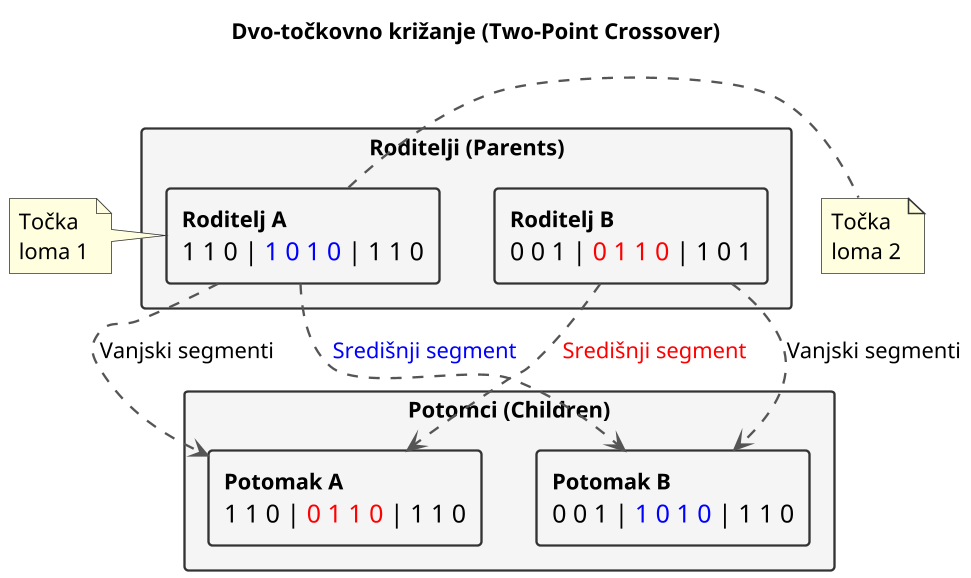
\includegraphics[width=0.8\textwidth]{slike/crossover_diagram.png}
    \caption{Vizualni prikaz operatora dvo-točkovnog križanja (Two-Point Crossover). Segmenti između dviju nasumično odabranih točaka loma se razmjenjuju između roditeljskih kromosoma kako bi se stvorili potomci.}
    \label{fig:crossover}
\end{figure}
\paragraph{Mutacija.} Mutacija je primarni mehanizam istraživanja i osigurava genetsku raznolikost. Ona nasumično mijenja pojedine gene u kromosomu s vrlo malom vjerojatnošću. Iako se može činiti kao destruktivan proces, Holland \cite{Holland1975} je naglasio njenu ključnu ulogu u sprječavanju prerane konvergencije, tj. situacije u kojoj cijela populacija postane previše slična i algoritam "zaglavi" u lokalnom optimumu.




\subsubsection{Više-kriterijski genetski algoritmi i NSGA-II}
\label{sec:NSGA-II}
Standardni genetski algoritmi dizajnirani su za probleme s jednim ciljem. Međutim, stvarni problemi, uključujući i odabir projektnog portfelja, inherentno su više-kriterijski. Njihov cilj nije pronaći jedno "najbolje" rješenje, već skup rješenja koji predstavlja optimalan kompromis, poznat kao Paretov front.

U svom utjecajnom radu, Deb i suradnici \cite{Deb2002} predstavili su \textbf{NSGA-II (\textit{Nondominated Sorting Genetic Algorithm II})} kao odgovor na tri ključna nedostatka tadašnjih više-kriterijskih algoritama: visoku računsku složenost, nedostatak elitizma i potrebu za specificiranjem dodatnih parametara. NSGA-II uvodi tri ključne inovacije koje rješavaju te probleme:

\begin{enumerate}
\item \textbf{Brzo sortiranje po nedominaciji:} Razvijen je značajno efikasniji algoritam za rangiranje populacije u slojeve (frontove) na temelju koncepta dominacije. Ovim se drastično smanjuje vrijeme potrebno za evaluaciju generacije, što je bila glavna prepreka u ranijim algoritmima.

\item \textbf{Eksplicitni elitizam:} Algoritam garantira da se najbolja rješenja pronađena u prethodnoj generaciji automatski prenose u sljedeću. Time se sprječava gubitak kvalitetnih rješenja do kojeg je moglo doći zbog stohastičke prirode genetskih operatora.

\item \textbf{Procjena gustoće naseljenosti (Crowding distance):} Umjesto specificiranja dodatnih parametara za održavanje raznolikosti, NSGA-II uvodi elegantan mehanizam "napučenosti". Unutar istog fronta, prednost se daje rješenjima koja se nalaze u rjeđe naseljenim dijelovima prostora rješenja. Time se osigurava da algoritam pronađe širok i dobro raspoređen Paretov front, pružajući donositelju odluke raznolik skup kompromisnih opcija.
\end{enumerate}

Zbog ove tri ključne prednosti – računalne efikasnosti, garantiranog elitizma i održavanja raznolikosti bez dodatnih parametara – NSGA-II je odabran kao temelj za više-kriterijski hibridni model u ovom radu.
\subsubsection{Izazov podešavanja parametara genetskog algoritma}

Performanse genetskog algoritma nisu ovisne samo o odabiru reprezentacije i operatora, već i o pažljivom podešavanju njegovih ključnih parametara. Najvažniji parametri uključuju:
\begin{itemize}
    \item \textbf{Veličina populacije (\texttt{POP\_SIZE}):} Određuje koliko se rješenja istovremeno istražuje. Veća populacija bolje pokriva prostor rješenja i čuva raznolikost, ali značajno povećava računsku zahtjevnost.
    \item \textbf{Broj generacija (\texttt{NGEN}):} Definira koliko dugo će evolucija trajati. Više generacija omogućuje algoritmu da duže konvergira prema optimumu, ali također povećava vrijeme izvođenja.
    \item \textbf{Vjerojatnost križanja (\texttt{CX\_PB}):} Kontrolira učestalost primjene operatora križanja. Visoka vrijednost potiče rekombinaciju i iskorištavanje postojećih rješenja.
    \item \textbf{Vjerojatnost mutacije (\texttt{MUT\_PB}):} Kontrolira učestalost mutacije. Niska vrijednost je ključna, jer prevelika mutacija pretvara algoritam u nasumičnu pretragu, dok premala može dovesti do prerane konvergencije.
\end{itemize}
Pronalaženje optimalne ravnoteže između ovih parametara je ključan i netrivijalan problem, jer ne postoji univerzalna konfiguracija koja radi dobro za sve probleme. Upravo iz tog razloga, prije provođenja glavnih eksperimenata, u ovom radu je provedena \textbf{ablacijska studija (Eksperiment 1)}, s ciljem empirijskog utvrđivanja "šampionske" konfiguracije parametara za specifičan problem koji se analizira.
\subsection{Kvantifikacija rizika pomoću Monte Carlo simulacije}
\label{sec:mcs}

Monte Carlo simulacija (MCS) je moćna računska metoda koja koristi ponovljeno nasumično uzorkovanje za numeričko modeliranje i analizu složenih, stohastičkih sustava. Iako su njeni korijeni vezani uz razvoj nuklearnog oružja sredinom 20. stoljeća \cite{Metropolis1949}, danas je postala nezamjenjiv alat u raznim disciplinama, od financija do inženjerstva, a posebno u kvantitativnoj analizi rizika \cite{Vose2008}. U kontekstu projektnog upravljanja, primjena MCS-a omogućuje prelazak s tradicionalnih, determinističkih planova na probabilističke modele koji realističnije oslikavaju nesigurnost ishoda projekta \cite{Miller2009, Avlijas2008}.

Temeljna vrijednost Monte Carlo simulacije, kako ističe Vose \cite{Vose2008}, leži u njenoj sposobnosti da transformira nesigurnost ulaznih varijabli u distribuciju vjerojatnosti izlaznih rezultata. Umjesto da projektni menadžer dobije jednu, često pogrešnu, točku procjene (npr. "projekt će trajati 350 dana"), MCS generira cijeli spektar mogućih ishoda (npr. histogram trajanja projekta). Analizom te izlazne distribucije moguće je donijeti puno informiranije odluke, odgovarajući na ključna pitanja poput: "Koja je vjerojatnost da ćemo završiti projekt unutar 400 dana?" ili "Koji je raspon trajanja u kojem se s 90\% pouzdanosti možemo očekivati završetak?".

Sam proces simulacije odvija se u nekoliko logičkih koraka. Prvo se identificiraju ključne ulazne varijable čije su vrijednosti neizvjesne, poput trajanja pojedinih aktivnosti. Za svaku takvu varijablu odabire se distribucija vjerojatnosti koja najbolje opisuje raspon i vjerojatnost njenih mogućih vrijednosti. Zatim, algoritam iterativno provodi tisuće "eksperimenata": u svakoj iteraciji, za svaku nesigurnu varijablu generira se jedna nasumična vrijednost iz njene definirane distribucije te se na temelju tih vrijednosti izračunava ishod modela (npr. ukupno trajanje projekta).

Pouzdanost ove metode, kako objašnjavaju Rubinstein i Kroese \cite{Rubinstein2016}, temelji se na fundamentalnom statističkom principu – Zakonu velikih brojeva. On jamči da će prosječna vrijednost rezultata dobivenih iz velikog broja neovisnih simulacija konvergirati prema stvarnoj očekivanoj vrijednosti sustava. Ponavljanjem procesa velik broj puta, dobiva se empirijska distribucija mogućih ishoda koja pruža dublji uvid od jedne determinističke procjene i iz koje se mogu iščitati ključni statistički pokazatelji poput očekivane vrijednosti, standardne devijacije i vjerojatnosti prekoračenja određenih pragova.
Njena matematička podloga leži u \textbf{Zakonu velikih brojeva}, koji garantira da će prosječna vrijednost rezultata dobivenih iz velikog broja simulacija konvergirati prema stvarnoj očekivanoj vrijednosti.
Proces monte carlo simulacije odvija se u nekoliko koraka. prvo se identificiraju ključne ulazne varijable čije su vrijednosti neizvjesne, poput trajanja pojedinih aktivnosti. za svaku takvu varijablu odabire se distribucija vjerojatnosti koja najbolje opisuje raspon i vjerojatnost njenih mogućih vrijednosti. zatim, algoritam iterativno provodi tisuće "eksperimenata": u svakoj iteraciji, za svaku nesigurnu varijablu generira se jedna nasumična vrijednost iz njene definirane distribucije, te se na temelju tih vrijednosti izračunava ishod modela (npr. ukupno trajanje projekta). ponavljanjem ovog procesa velik broj puta, dobiva se empirijska distribucija mogućih ishoda koja pruža dublji uvid od jedne determinističke procjene i iz koje se mogu iščitati ključni statistički pokazatelji poput očekivane vrijednosti, standardne devijacije i vjerojatnosti prekoračenja određenih pragova.

\subsection{Modeliranje nesigurnosti trajanja pomoću trotočkovne procjene}
\label{sec:triangular}
Metodologija PERT (\textit{Program Evaluation and Review Technique}) uvela je u praksu korištenje tri vremenske procjene za aktivnosti s neizvjesnim trajanjem, što je danas standard u upravljanju projektnim rizikom \cite{Malcolm1959}. Ove tri točke su: $T_o$(optimistična procjena), $T_m$(najvjerojatnija procjena) i $T_p$(pesimistična procjena).

Dok tradicionalna PERT metoda koristi ove tri točke za izračun parametara Beta distribucije, u modernoj praksi, a posebno u Monte Carlo simulacijama, često se koristi \textbf{Trokutasta distribucija} zbog svoje jednostavnosti i intuitivnosti \cite{Law2015}. 

Averill Law, u svom seminalnom djelu "Simulation Modeling and Analysis" (2015), pozicionira trokutastu distribuciju kao iznimno pragmatičan i koristan alat, osobito u situacijama kada nedostaju detaljni povijesni podaci te se modeliranje mora osloniti na stručne procjene. Njena glavna snaga leži u intuitivnosti, jer direktno koristi tri točke procjene (minimum, maksimum i najvjerojatnija vrijednost) koje su lako razumljive i procjenjive od strane projektnih menadžera i inženjera bez dubljeg statističkog znanja. Uz to, njena matematička jednostavnost i definirani interval čine je računski efikasnom i prikladnom za modeliranje realnih veličina poput trajanja aktivnosti, koje ne mogu poprimiti negativne ili beskonačne vrijednosti. Kod trokutaste distribucije i funkcija gustoće vjerojatnosti (PDF) i kumulativna funkcija distribucije (CDF) su matematički jednostavne (sastoje se od linearnih i kvadratnih segmenata), što je čini računalno vrlo "jeftinom" i lakom za implementaciju u simulacijskim alatima. 

Unatoč ovim praktičnim prednostima, Law također upozorava na njene teorijske limite. Ističe da je linearni oblik distribucije često proizvoljna pretpostavka koja možda ne odražava u potpunosti stvarni proces, jer  postoji fundamentalni razlog zašto bi se vjerojatnost smanjivala točno linearno od najvjerojatnije vrijednosti prema ekstremima. Stvarni procesi često imaju "zaobljenije" distribucije. Uz to, srednja vrijednost i varijanca distribucije su iznimno osjetljive na procjene minimuma ($a$) i maksimuma ($b$). Rezultati simulacije mogu biti osjetljivi na nerealno pesimistične ili optimistične krajnje točke koje definira stručnjak. Zbog toga je iznimno važno kritičko propitivanje ekstremnih procjena. Ipak, Law zaključuje da je, unatoč postojanju matematički elegantnijih alternativa poput Beta distribucijom koja se tradicionalno koristi u PERT analizi (dok trokutasta ima oštre vrhove i ravne linije, Beta distribucija (kada se definira s istim parametrima) ima glađi, zaobljeniji oblik koji mnogi smatraju realističnijim) , trokutasta distribucija zbog svoje robusnosti i praktičnosti legitiman i često preferiran izbor u praksi upravljanja rizikom, predstavljajući obranjiv inženjerski pristup modeliranju nesigurnosti.

Ukratko, trokutasta distribucija je kontinuirana distribucija vjerojatnosti definirana s tri parametra: minimum ($a$), maksimum ($b$) i najvjerojatnija vrijednost ($c$), što direktno odgovara procjenama $T_o$, $T_p$ i $T_m$. Njena je glavna prednost što ne zahtijeva opsežne povijesne podatke, već se može temeljiti na stručnom iskustvu, što je čini iznimno pogodnom za projektno planiranje. Slučajne vrijednosti generirane iz ove distribucije nalaze se unutar intervala [$T_o$, $T_p$], s najvećom vjerojatnošću pojavljivanja oko vrijednosti $T_m$.  Taj konačni interval ključan je za modeliranje realnih pojava. Prosječna vrijednost (očekivano trajanje) za Trokutastu distribuciju računa se jednostavnom formulom:

$$
E(T) = \frac{T_o + T_m + T_p}{3}
$$

Upravo je Trokutasta distribucija, zbog svih navedenih prednosti, odabrana kao temelj za modeliranje nesigurnosti trajanja aktivnosti u Monte Carlo simulacijama provedenim u ovom radu.
